%!TEX root = farm.tex


\section{Experiments}\label{sec:evaluation}

We now evaluate the basic performance of the firmware developed using
our compiler and debugging environment.
We also discuss what we have found in our experiments.

\subsection{Performance Evaluation}

\begin{table}[!t]
 \caption{Experimental setup.} 
 \label{tab:environment}
 \hbox to\hsize{\hfil
 \begin{tabular}{|l|l|}\hline
  CPU &  Intel core i7 2600 \\\hline
  GPU &  NVIDIA GeForce GTX480 \\\hline
  Memory & 8GB \\\hline
  Kernel & Linux 2.6.42.12-1.fc15.x86\_64 \\\hline
  Device driver & Gdev~\cite{Kato_ATC12} \\\hline
 \end{tabular}\hfil}
\end{table}

We evaluate the performance of our firmware as compared with NVIDIA's
proprietary firmware blob.
Table~\ref{tab:environment} shows our experimental setup.
For fair comparison, we use Gdev~\cite{Kato_ATC12} as the underlying GPU
device driver and runtime, given that our firmware is available for only
the open-source environment.
The performance metric of our experiments is a total execution time
including GPU executions and data transfers between the host and the
device.

\begin{figure}
 \begin{center}
  \hfil
  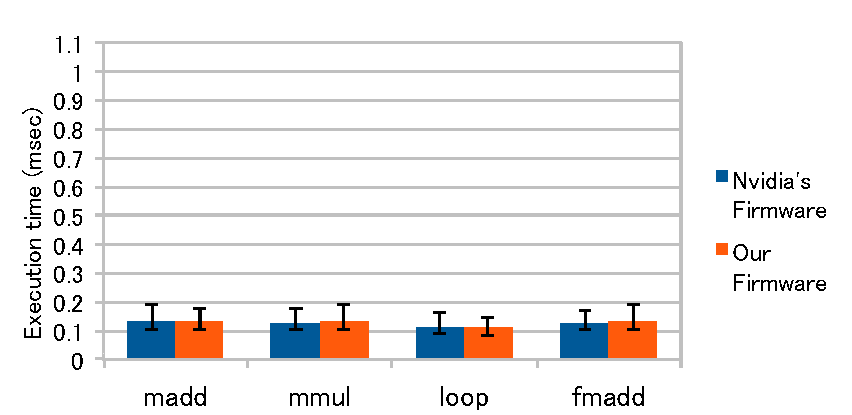
\includegraphics[width=8cm]{./img/good_case.pdf}
 \end{center}
 \caption{Execution time of microbenchmark programs: Case (i).}
 \label{fig:goodcase}
\end{figure}

\begin{figure}
 \begin{center}
  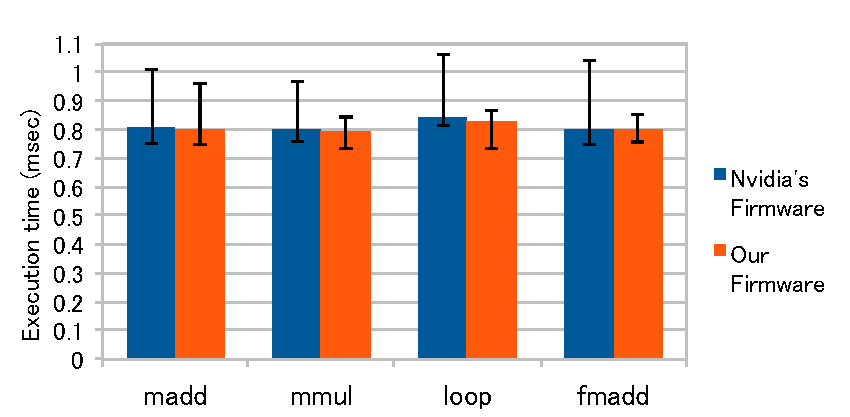
\includegraphics[width=8cm]{./img/bad_case.pdf}
 \end{center}
 \caption{Execution time of microbenchmark programs: Case (ii).}
 \label{fig:badcase}
\end{figure}

To average variations in the execution time, we run each test program 100
times.
Our observation is that our firmware and NVIDIA's firmware exhibit
similar behavior - the execution time is mostly less than 2 $ms$ or more
than 7 $ms$. 
We hence categorize them into two cases: (i) less than 2 $ms$ and (ii)
more than 7 $ms$.
Figures~\ref{fig:goodcase} and \ref{fig:badcase} depict the experimental
results of these two cases, respectively, where the X axis lists our
microbenchmark programs and the Y axis shows their execution time.

As can be seen from the experimental results, the performance difference
between our firmware and NVIDIA's firmware is very trivial in Case (i).
For example, it is at most 0.003 $ms$ in the madd program, which is
equivalent to 2.31\% of the time.
In the case (ii), on the other hand, our firmware rather outperforms
NVIDIA's firmware by 0.002 $ms$, i.e., 1.74\% of the time.
Such a performance difference, however, is negligible due to the
following reasons.
\begin{itemize}
 \item The observed performance difference is much smaller than their
       error margin.
 \item The total execution time is occupied by GPU executions rather
       than firmware execution.
       For instance, the total execution time of the madd program under
       NVIDIA's firmware is 21.842 $ms$, which is mostly dominated by the
       host-side execution, whereas the firmware execution time is no
       greater than 0.01\% of the total execution time. 
\end{itemize}

The above experimental results imply that our compiler and debugging
environment for NVIDIA's GPU microcontrollers is reliable in
performance.
Given that firmware developers can use C language rather than hand
assembling, we believe that the contribution of this paper is
significant in this line of work.

\subsection{Discussions}

Through the experiment, we observed that the execution time of the madd
program was 214 $ms$ at the first trial, while that after the second
time is around 20 $ms$.
We found out that this big gap comes from the fact that the firmware has
to generate the GPU context at the first run, while it can reuse the
same context information from the second run.
This explains the cost of generating the GPU context.
Without self-firmware development, we would have never have these
findings.


